% !TeX spellcheck = it_IT
\documentclass{llncs}
%%%%%%%%%%%%%%%%%%%%%%%%%%%%%%%%%%%%%%%%%%%%%%%%%%%%%%%%%%%
%% package sillabazione italiana e uso lettere accentate
\usepackage[latin1]{inputenc}
\usepackage[english]{babel}
\usepackage[T1]{fontenc}
%%%%%%%%%%%%%%%%%%%%%%%%%%%%%%%%%%%%%%%%%%%%%%%%%%%%%%%%%%%%%

\usepackage{url}
\usepackage{xspace}
\usepackage{amsmath}
\usepackage{pdfpages}


\makeatletter
%%%%%%%%%%%%%%%%%%%%%%%%%%%%%% User specified LaTeX commands.
\usepackage{manifest}
\usepackage{listings}
\usepackage{textcomp}
\makeatother

\usepackage{tikz}
\usetikzlibrary{arrows,automata}

\newcommand{\java}{\textsf{Java}}
\newcommand{\contact}{\emph{Contact}}
\newcommand{\corecl}{\texttt{corecl}}
\newcommand{\medcl}{\texttt{medcl}}
\newcommand{\msgcl}{\texttt{msgcl}}
\newcommand{\android}{\texttt{Android}}
\newcommand{\dsl}{\texttt{DSL}}
\newcommand{\jazz}{\texttt{Jazz}}
\newcommand{\rtc}{\texttt{RTC}}
\newcommand{\ide}{\texttt{Contact-ide}}
\newcommand{\xtext}{\texttt{XText}}
\newcommand{\xpand}{\texttt{Xpand}}
\newcommand{\xtend}{\texttt{Xtend}}
\newcommand{\pojo}{\texttt{POJO}}
\newcommand{\junit}{\texttt{JUnit}}

\newcommand{\action}[1]{\texttt{#1}\xspace}
\newcommand{\code}[1]{{\small{\texttt{#1}}}\xspace}
\newcommand{\codescript}[1]{{\scriptsize{\texttt{#1}}}\xspace}

% Cross-referencing
\newcommand{\labelsec}[1]{\label{sec:#1}}
\newcommand{\xs}[1]{\sectionname~\ref{sec:#1}}
\newcommand{\xsp}[1]{\sectionname~\ref{sec:#1} \onpagename~\pageref{sec:#1}}
\newcommand{\labelssec}[1]{\label{ssec:#1}}
\newcommand{\xss}[1]{\subsectionname~\ref{ssec:#1}}
\newcommand{\xssp}[1]{\subsectionname~\ref{ssec:#1} \onpagename~\pageref{ssec:#1}}
\newcommand{\labelsssec}[1]{\label{sssec:#1}}
\newcommand{\xsss}[1]{\subsectionname~\ref{sssec:#1}}
\newcommand{\xsssp}[1]{\subsectionname~\ref{sssec:#1} \onpagename~\pageref{sssec:#1}}
\newcommand{\labelfig}[1]{\label{fig:#1}}
\newcommand{\xf}[1]{\figurename~\ref{fig:#1}}
\newcommand{\xfp}[1]{\figurename~\ref{fig:#1} \onpagename~\pageref{fig:#1}}
\newcommand{\labeltab}[1]{\label{tab:#1}}
\newcommand{\xt}[1]{\tablename~\ref{tab:#1}}
\newcommand{\xtp}[1]{\tablename~\ref{tab:#1} \onpagename~\pageref{tab:#1}}
% Category Names
\newcommand{\sectionname}{Section}
\newcommand{\subsectionname}{Subsection}
\newcommand{\sectionsname}{Sections}
\newcommand{\subsectionsname}{Subsections}
\newcommand{\secname}{\sectionname}
\newcommand{\ssecname}{\subsectionname}
\newcommand{\secsname}{\sectionsname}
\newcommand{\ssecsname}{\subsectionsname}
\newcommand{\onpagename}{on page}

\newcommand{\student}{Gruppo 3 Aimi Niccol\'o, Gallegati Mattia, Murgia Antonio, Zanotti Andrea }
\newcommand{\studentEmail}{niccolo.aimi@studio.unibo.it; mattia.gallegati2@studio.unibo.it; antonio.murgia2@studio.unibo.it; andrea.zanotti9@studio.unibo.it}
\newcommand{\xfaculty}{II Faculty of Engineering}
\newcommand{\xunibo}{Alma Mater Studiorum -- University of Bologna}
\newcommand{\xaddrBO}{viale Risorgimento 2}
\newcommand{\xaddrCE}{via Venezia 52}
\newcommand{\xcityBO}{40136 Bologna, Italy}
\newcommand{\xcityCE}{47023 Cesena, Italy}

%
% Comments
%
%%% \newcommand{\todo}[1]{\bf{TODO:}\emph{#1}}


\begin{document}

\title{Final Theme System\\
 process report}

%%% \author{\xauthA \and \xauthB}
\author{\student}

\institute{%
%%%  \xunibo\\\xaddrCE, \xcityCE\\\email{\{nameA.studentA, nameB.studentB\}@studio.unibo.it}
  \xunibo\\\xaddrBO, \xcityBO\\\email\ {\studentEmail}
}

\maketitle

%% \begin{abstract}
%% \footnotesize
%%This a Latex template to be used for the reports of Software Engineering.
%%\keywords{Software engineering, managed software development, reports, ....}
%%\end{abstract}

%%% \sloppy

%===========================================================================
\section{Introduction}
\labelsec{intro}
In this document we'll describe and discuss the process that led to the development of a robotic software system. We'll discuss how traditional software/project development techniques can and should merge with the scrum project management system.\\ 
We'll face the limits of traditional analysis approaches and purpose novel ones that better match with new programming paradigms.
%===========================================================================

%===========================================================================
\section{Vision}
\labelsec{Vision}
Here we're collecting some visions that will inspire the development of this project and of software in general:\\
\begin{itemize}
	\item There's no code without project, there's no project without problem analysis and there's no problem without requirements;
	\item There's no code without tests. That means that tests must be developed before the development of the software product;
	\item There's no code without documentation;
	\item The team that develops the tests should be different from the one who will realize the project;
	\item We should use a top down approach during the development phase and bottom-up approach during the implementation phase;
	\item Zooming? Trying to get closer..
		We should look at things initially from a far point of view like a black box and then trying to get closer to the details of the system, white box.
	\item Any sufficiently advanced technology is indistinguishable from magic.
	\item Develop the code in an IOT prospective using the ICT principles.
	\item Create valuable software using less time and resource possible in order to optimize software development process (factorization).
	\item A feature does not exist unless a test validates that it functions.
	\item Software entities should be open for extension but closed for modification.
	\item We should always check the existence of prior projects, trends or patterns regarding the technological domain we are facing. If does exist something we should study it, not only to take advantage of it during the development but also to recognize its limits and to purpose some innovative approach coming from different technological domains;
	\item The development of the project should be technology agnostic;
	\item We should find or create a formal language able to describe the results of the problem analysis. It should be similar to spoken language. This language could take advantage of different programming paradigms (functional, declarative and so on) and different programming models (actor model, message passing model and so on). This language should not be tied to any technology implementation. There should be one or more parsers/compilers for this language that will generate source code for a specific platform. This generated code should be used as the skeleton of the real product.
\end{itemize}
%===========================================================================

%===========================================================================
\section{Goals}
\section{Goals}
\labelsec{Goals}
The first goal is to develop a robotic software system using the most advanced programming paradigms.\\ 
A secondary goal is to develop and to take advantage of a novel technique of requirements and problem analysis that will lead to a formal representation of the problem and to source code generation.
Finally the main goal is discuss how some change (monotonic extensions) of the requirements impact on a product whose production is based on 'formal' and 'technology independent' artifacts rather than on ad-hoc code.
\labelsec{Goals}
%===========================================================================

%===========================================================================
\section{Requirements}
\labelsec{Requirements}
Design and build a (prototype of a) software system that, with reference to a differential drive robot (called from now on robot):
\begin{itemize}
	\item allows a user to select between a 'learning phase' and a 'autonomous phase'
    during the learning phase, the user can send a sequence of move commands (e.g. forward, backward, left right, stop) to the robot. The robot must not only execute each command but it must also record the whole sequence of commands until the user decides to terminate the learning phase;
    \item after the termination of the learning phase, the user can tell the robot to enter the autonomous phase in a 'direct' or in a 'reverse' mode. During this phase the robot executes in autonomous way the sequence of moves it has learned, by complementing each move (e.g. forward->backward) if the selected mode is reverse;
    \item during the autonomous phase, the robot must be able to execute (as soon as possible) a stop command sent by the user.
\end{itemize}
After the development of this prototype, consider the possibility to enhance the functional capabilities of the robot, by allowing it:
\begin{itemize}
	\item to perceive an obstacle during the autonomous phase and, once the obstacle is detected, to execute some alternative behaviour (in term of moves).
\end{itemize}

%===========================================================================

 
%===========================================================================
\section{Requirement analysis}
\labelsec{ReqAnalysis}
%===========================================================================
\subsection{Use cases}
creo con visio omarino con tutti gli ovali con le possibilit�
\labelssec{UseCases}

\subsection{Scenarios}
\labelssec{Scenarios}

\subsection{(Domain)model}
\labelssec{(Domain)model}
\paragraph{Structure}
\subsubsection{ROBOT}
We consider the robot as a reactive and atomic entity.
\subsubsection{REMOTE}
We consider the remote as a proactive and atomic entity.
\paragraph{Interaction}
The interaction between the entities of the system is described with this sequence diagram:
\begin{center}
   	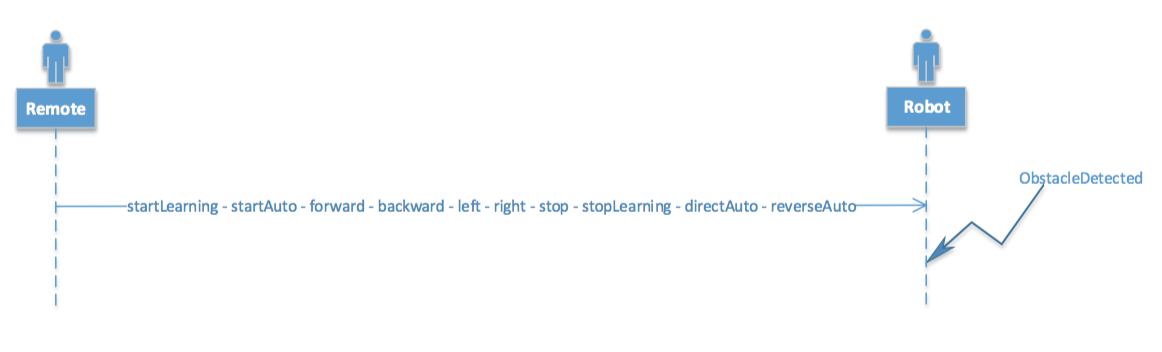
\includegraphics[width=13cm]{img/interactionRobot.png}\\
\end{center}
\paragraph{Behaviour}
\subsubsection{ROBOT}
The behaviour of the robot is described with this FSM:\\
\begin{center}
   	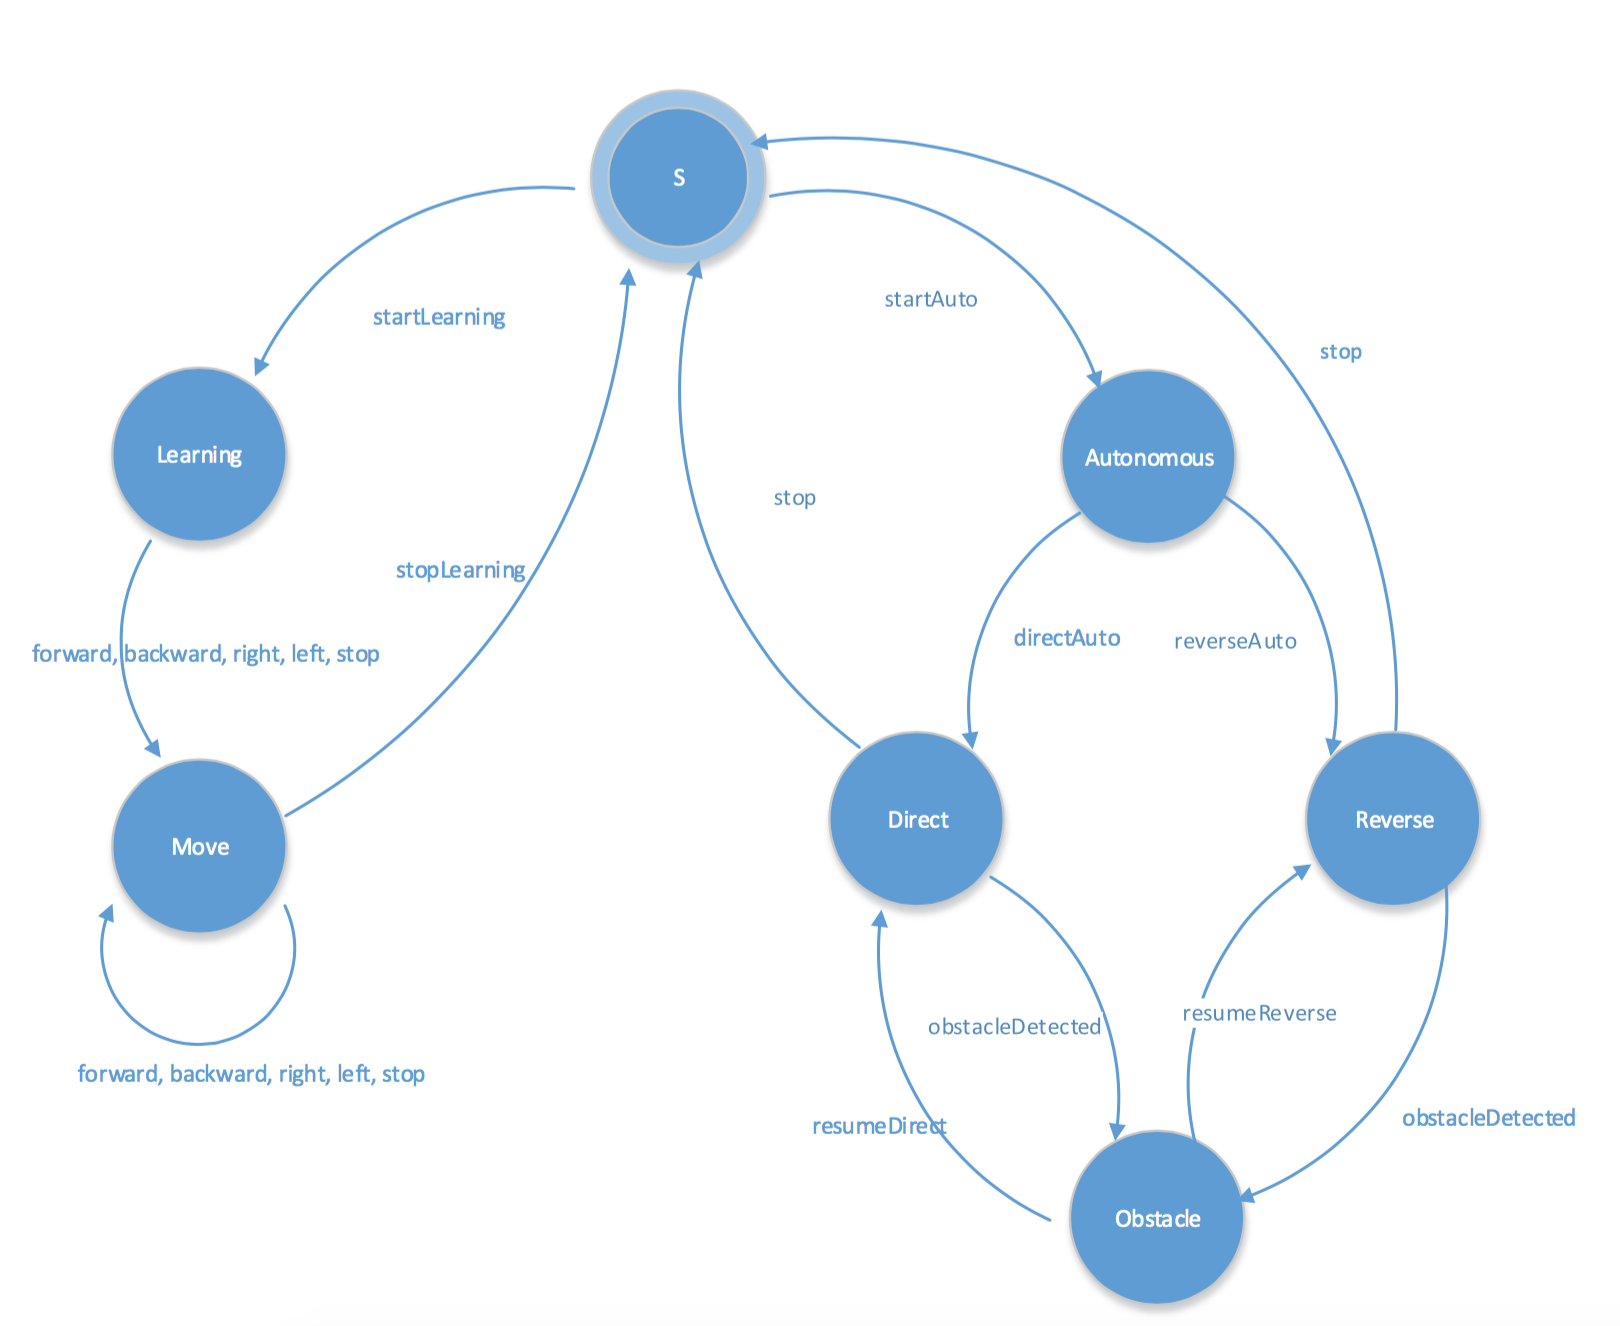
\includegraphics[width=12.5cm]{img/fsmRobot.png}\\
\end{center}
\subsubsection{REMOTE}
The behaviour of the remote is described with this FSM:\\
\begin{center}
   	
\includegraphics[width=2cm]{img/fsmRemoteRequirementAnalysis.png}\\
\end{center}
\subsection{Test plan}
Test sui piani del robot e eventi remote
\labelsec{Test plan}
%===========================================================================
\section{Problem analysis}
\labelsec{ProblemAnalysis}
Our technological hypothesis is JAVA and Object Oriented Programming. We will show that we need to develop a new infrastructure because the only features offered by the programming language chosen are not sufficient.  
To mantain our code well developed, scalable, efficient and mantainable, we will use the most known development patterns.
%
\`E inoltre necessario accordarsi su un linguaggio di interazione, il quale necessita di uno standard di comunicazione. Lo standard di comunicazione sar\`a indispensabile per Integration Test.
%===========================================================================
\subsection{Abstraction gap}
We discovered that our unique tool in Java is procedure calls communication, so with the OO paradigm we can't realize a modular communication where entities are completely independent. We need a new way to let our components interact.
In agreement with our vision, we understand that the best way to overcome this problem is to develop a new software infrastructure that will be more useful than Java paradigms.
This infrastructure will be used not only in this project, but every future developed process that will have the same needs.\\
Our platform must reach some main goals: 
\begin{itemize}
\item Model driven programming in order to generate useful code starting from some formal rappresentation of our model (QA file). 
\item Message based communication in order to transfer information in asynchronous or synchronous way. 
\item A new formal executing entity that must be able to:\\ 
1)Execute plans of actions.\\
2) Receive message from other entities.\\ 
3) Store information in a private queue in order to receive all the messages (Message Based). 
\end{itemize}
We want to be on top of the distribution of our system, in order to reach that goal we can think that every entity lives in a context. Every context contains one or more entities that can use easy forms of communication without paying remote communication costs. They can also communicate from a context to another using remote communication based on message passing.
In order to introduce a new form of communication that is not strictly point to point we can introduce a new concept : Events.\\
Events are a form of asynchronous communication that is not point to point. In our system our entities can declare to be interested in an event, when that event will be emitted the entities must react in some way.
We introduce also a new behavior for our entities: the FSM. If an entity is modeled as a FSM it will have different State configurations, every state is connected to other states with its own logic, it could be event driven or not.
We also need to introduce asynchronous actions. Asynchronous actions are operations that need a considerable time to be executed, their execution can be made in a blocking or non blocking manner. Instead of managing them with callback programming we decide to make actions realiably interrupted by selected events and to handle those events with chosen routines. Those routines have to specify if after their execution the previous asynchronous action must be resumed or stopped.
\subsection{Logic architecture}
L'architettura logica \`e esplicitata in figura.
\begin{center}
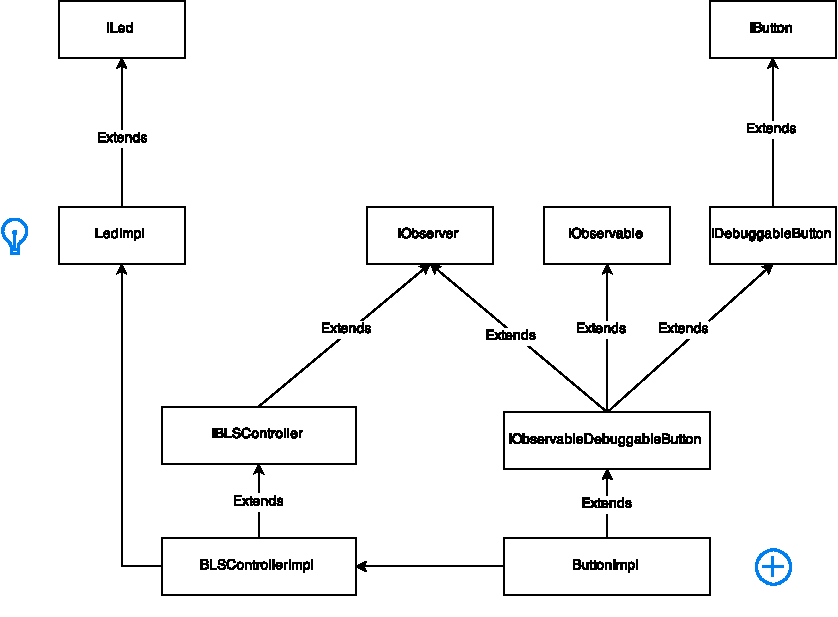
\includegraphics{img/graphs/Analisi_BLS.pdf}
\end{center}
\begin{center}

\end{center}

\subsection{Risk analysis}
Nell'interfaccia del Button, oltre al metodo accessor \texttt{isPressed} deve essere presente anche il metodo \texttt{addObserver}, ci\`o \`e risultato necessario dai colloqui con il committente (durante l'analisi dei requisiti).
%===========================================================================
\section{Work plan}
\labelsec{wplan}
%===========================================================================

%===========================================================================
\section{Project}
\labelsec{Project}
L'architettura progettuale \`e esplicitata in figura.\\
\url{https://github.com/iBelliDiISS/ButtonLedJava}
\begin{center}
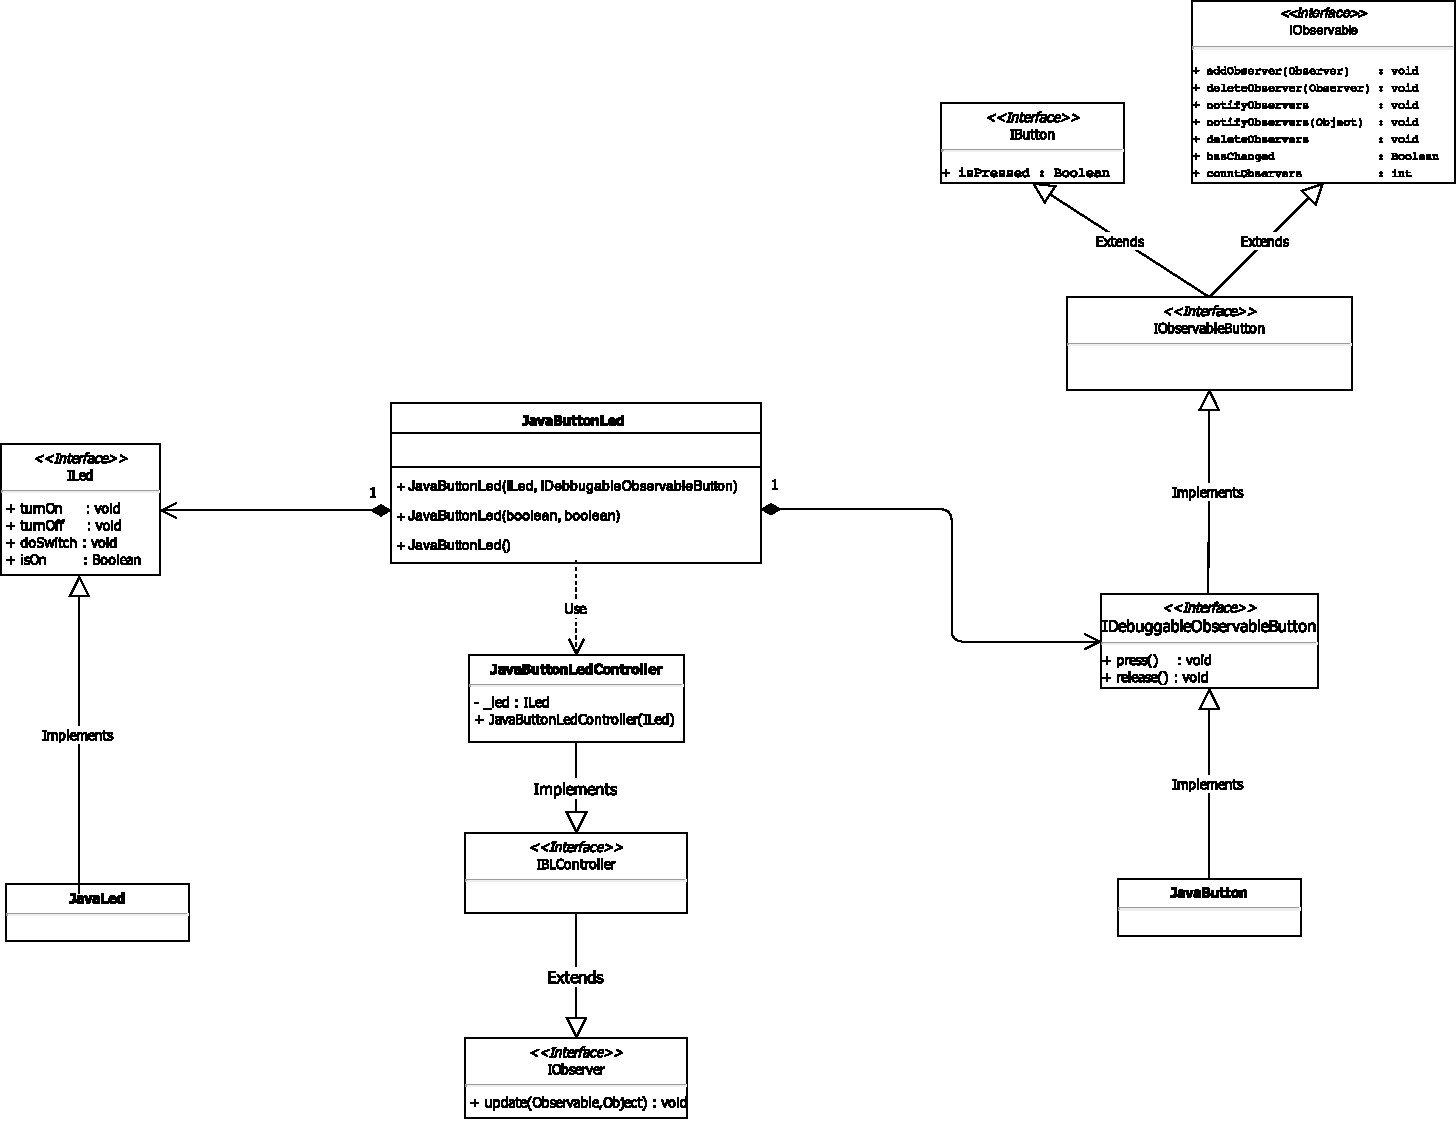
\includegraphics[scale=0.6]{img/graphs/Progettazione_BLS.pdf}
\end{center}
%===========================================================================

\subsection{Structure}
\subsection{Interaction}
\begin{center}
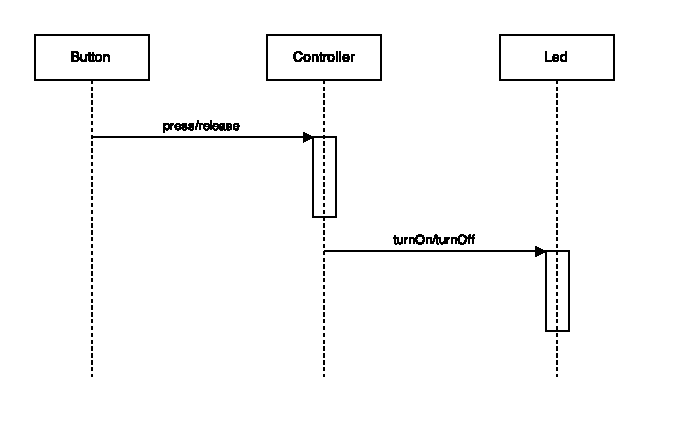
\includegraphics{img/graphs/Interaction.pdf}
\end{center}
\subsection{Behavior}
%===========================================================================
\section{Implementation}
\labelsec{Implementation}
%===========================================================================

%===========================================================================
\section{Testing}
\labelsec{testing}
%===========================================================================

%===========================================================================
\section{Deployment}
\labelsec{Deployment}
%===========================================================================

%===========================================================================
\section{Maintenance}
\labelsec{Maintenance}
%===========================================================================

%===========================================================================
\section{Discussion}
\paragraph{Requirement analysis}

\labelsec{Discussion}
%===========================================================================
discutere dell'evento nel caso sia generato dal nulla o da altro
dire come rappresentarlo visto che non possiamo farlo in uml
introduzione del sistema ad attori rispetto a java
problema se in analisi dei requisiti parlare dell'indipendenza dalla tecnologia
cambiamento dell'fsm del remote in fase successiva
%===========================================================================
\newpage
\appendix
\section{Codice}
\section{Information about the author}
\labelsec{Author}
%===========================================================================
\appendix
%===========================================================================
\vskip.5cm
%%% \begin{figure}
\begin{tabular}{ | c |  }
	\hline
	Photo of the Author\\
   	
\includegraphics[width=5cm]{img/zano.jpg}\\
	\hline
\end{tabular}
 
\appendix


\bibliographystyle{abbrv}
\bibliography{biblio}

\end{document}












